
\section{第~7~章的练习}
\label{sec:ch14-exercises-ch7}

\vkexsync{35}%

\begin{exercise}\label{ex:ch14-035-symplectic-transvection}
关系式 ${}^tAJ_0A=J_0$ 对一个\trSymplectic{}矩阵 $A$ 的行列式意味着什么？

为了证明这个行列式是 $+1$，我们可以仿照\cref{subsec:polar-decomposition}中的做法。另一种方法则在于证明\trSymplecticGroup{}由映射
\[
x\longmapsto x+\lambda\,\omega(x,a)\,a
\]
（\textbf{\trSymplecticTransvection}（symplectic transvection））所生成。本练习请你做的正是这件事。
\end{exercise}

\begin{exercise}\label{ex:ch14-036-rho-transvection}
设 $T$ 是一个\trSymplecticTransvection（\cref{ex:ch14-035-symplectic-transvection}）。计算 $\rho(T)$。映射 $\rho$ 是否满足
\[
\rho(AB)=\rho(A)\rho(B)\text{？}
\]
\end{exercise}

\begin{exercise}[$\mathrm{U}(n)$ 的\trFundamentalGroup]\label{ex:ch14-037-fundamental-group-un}
群 $\mathrm{SU}(n)$ 作用于单位\trSphere{} $S^{2n-1}\subset\CC^{n}$，其作用方式使得\trCanonical{}基最后一个向量的\trStabilizer{}\footnote{译注：原书此处印作 “the stabilizer the last vector”；按文义疑漏介词 of，应为 “the stabilizer of the last vector”；此处径补。——译者注}可以与 $\mathrm{SU}(n-1)$ 相等同。由此推出：$\mathrm{SU}(n)$ 是\trSimplyConnected{}的。

证明：映射
\[
\mathrm{U}(n)\xrightarrow{\ \det\ }S^{1}
\]
在\trFundamentalGroup{}上诱导一个\trIsomorphism。
\end{exercise}

\begin{exercise}\label{ex:ch14-038-maslov-path-examples}
考虑矩阵
\[
A(t)=\begin{pmatrix}1+4\pi^{2}t^{2} & 2\pi t\\[2pt] 2\pi t & 1\end{pmatrix}
\qquad(t\in[0,1])\text{。}
\]
验证：道路 $t\mapsto A(t)$ 落在 $\scr{S}$（定义见\cref{subsec:first-step}）之中，并计算它的\trMaslovIndex。

对矩阵
\[
A(t)=\begin{pmatrix}1-4\pi^{2}t^{2} & -2\pi t\\[2pt] 2\pi t & 1\end{pmatrix}
\qquad(t\in[0,1])\text{。}
\]
做同样的事（这更为微妙）。
\end{exercise}

\begin{exercise}\label{ex:ch14-039-rho-jordan-block}
在配备了坐标 $(q_1,q_2,p_1,p_2)$ 的 $\RR^{4}$ 中，赋予\trSymplecticForm{}
$\omega=dp_1\wedge dq_1+dp_2\wedge dq_2$ 与\trComplexStructure{}
$J=\begin{pmatrix}0&\mathrm{Id}\\-\mathrm{Id}&0\end{pmatrix}$，考虑\trQuadraticForm
\[
H=\frac{1}{2}\bigl(p_1^{2}+p_2^{2}\bigr)+(q_2p_1-q_1p_2)
\]
以及相伴的\trSymmetricMatrix\footnote{译注：原书此处左下块亦印作 $-\alpha$（两块均 $-\alpha$）；由右端显式 $4\times4$ 矩阵（或由 $S$ 对称而 $\alpha^{t}=-\alpha$）可知左下块应为 $\alpha$；此处径改。——译者注}
\[
S=\begin{pmatrix}
0&0&0&-1\\
0&0&1&0\\
0&1&1&0\\
-1&0&0&1
\end{pmatrix}
=\begin{pmatrix}0&-\alpha\\ \alpha&\mathrm{Id}\end{pmatrix}
\qquad\text{其中 }\alpha=\begin{pmatrix}0&1\\-1&0\end{pmatrix}\text{。}
\]
证明：
\[
A=\exp(tJS)=\begin{pmatrix}\exp(t\alpha) & t\exp(t\alpha)\\[2pt] 0 & \exp(t\alpha)\end{pmatrix}
=\begin{pmatrix}
\cos t & -\sin t & t\cos t & -t\sin t\\
\sin t & \cos t & t\sin t & t\cos t\\
0 & 0 & \cos t & -\sin t\\
0 & 0 & \sin t & \cos t
\end{pmatrix}\text{，}
\]
这是一个\trSymplectic{}矩阵，具有（二重的）\trEigenvalue{} $e^{\pm it}$；当 $t\neq0$ 时它不\trDiagonalizable，并且当 $t\neq0$ 时它属于 $\mathrm{Sp}(2n)^{+}$。\footnote{译注：本段照原书排印，有三点须留意。其一，按 $\alpha$ 的定义，$\exp(t\alpha)=\begin{pmatrix}\cos t&\sin t\\-\sin t&\cos t\end{pmatrix}$，而右端显式 $4\times4$ 矩阵的诸 $2\times2$ 块是 $\begin{pmatrix}\cos t&-\sin t\\\sin t&\cos t\end{pmatrix}$，两者旋转方向相反（后者相应于 $-\alpha$）。其二，下条 (2) 中 $X=(1,-i,0,0)$ 属于\trEigenvalue{} $e^{it}$ 的特征空间之说只与所印显式矩阵\trCompatible；若按 $\exp(t\alpha)$ 计算，$e^{it}$ 的特征向量应为 $(1,i,0,0)$。其三，“当 $t\neq0$ 时属于 $\mathrm{Sp}(2n)^{+}$”在 $t\in2\pi\ZZ$ 处失效：此时 $\exp(t\alpha)=\mathrm{Id}$，$\det(A-\mathrm{Id})=0$，$A$ 连 $\mathrm{Sp}(2n)^{\star}$ 都不属于，该断言应限 $t\notin2\pi\ZZ$。不过 (2) 的结论 $\rho(A)=1$ 只依赖于 $\operatorname{Im}\,\omega(\overline{X},X)=0$，与旋转方向的取舍无关。此处照原书排印，存疑备案。——译者注}

其次，计算 $\rho(A)$（对 $t\in\,]0,\pi[\,$）：
\begin{enumerate}[label=(\arabic*)]
\item 证明：$m_0=0$，并且 $\rho(A)=\bigl(e^{it}\bigr)^{\sigma}$，其中 $\sigma$ 是 $Q$ 在对应于\trEigenvalue{} $e^{it}$ 的那个特征空间 $E$ 上的\trSignature。
\item 证明：$X=(1,-i,0,0)\in E$，并且 $\operatorname{Im}\,\omega(\overline{X},X)=0$。由此推出：$\sigma=0$，从而 $\rho(A)=1$。
\end{enumerate}
\end{exercise}

\begin{exercise}[\trLagrange{}\trGrassmann\trManifold]\label{ex:ch14-040-lagrangian-grassmannian}
考虑 $\RR^{2n}=\CC^{n}$ 的\trLagrange{}式向量子空间所成的空间 $\Lambda_n$。证明：群 $\mathrm{U}(n)$ 传递地作用于 $\Lambda_n$，并且
\[
\RR^{n}=\bigl\{X\in\CC^{n}\ \bigm|\ \operatorname{Im}(X)=0\bigr\}
\]
的\trStabilizer{}与\trOrthogonal{}群 $\mathrm{O}(n)$ \trIsomorphic。由此推出：$\Lambda_n$ 是一个维数为 $n(n+1)/2$ 的\trConnected\trCompact\trManifold。

证明：映射
\[
\det\nolimits^{2}\colon\mathrm{U}(n)\longrightarrow S^{1}
\]
定义了一个从 $\Lambda_n$ 到 $S^{1}$ 的连续映射，并且它在\trFundamentalGroup{}上诱导一个\trIsomorphism。
\end{exercise}

\begin{exercise}[\trLagrange{}式\trImmersion{}的\trMaslov{}类]\label{ex:ch14-041-maslov-class-immersion}
设
\[
f\colon L\longrightarrow\RR^{2n}
\]
是一个把维数为 $n$ 的\trManifold{}映入 $\RR^{2n}$ 的\trImmersion。\footnote{译注：原书此处箭头右端印作 $\RR^{n}$；按同句后半“in $\mathbf{R}^{2n}$”及\trLagrange{}式\trImmersion{}的定义，疑漏上标 $2$，应为 $\RR^{2n}$；此处径改。——译者注}
假设 $f$ 是\trLagrange{}式的，也就是说，$f^\star\omega=0$；或者等价地，对 $L$ 中的每个 $x$，$T_xf(T_xL)$ 都是 $\RR^{2n}$ 的一个\trLagrange{}式子空间。

于是，把每个点送到该点处的\trTangentSpace，便定义了一个“高斯”映射 $\gamma(f)\colon L\to\Lambda_n$。复合
\[
\gamma(f)_\star\colon\pi_1(L)\longrightarrow\pi_1(\Lambda_n)=\ZZ
\]
从而把 $L$ 的每个\trLoop{}送到一个整数：即它的\trMaslov{}类。确定由\cref{fig:maslov-class-immersions}中的图形所定义的那些（\trLagrange{}式的）$S^{1}$ 到 $\RR^{2}$ 的\trImmersion{}的\trMaslov{}类。证明：一个\trEmbedding{}的\trCircle{}的\trMaslov{}类是 $\pm2$（使用“切线转动”定理；参见 [8]）。
\end{exercise}

\setcounter{figure}{2}%
\begin{figure}[htbp]
\centering
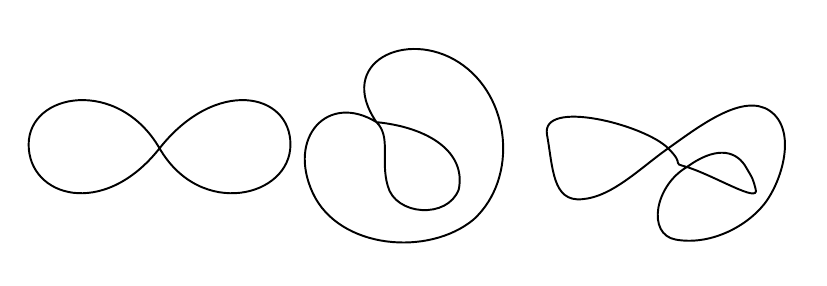
\begin{tikzpicture}[line width=0.7pt,scale=0.95]
  \begin{scope}[xshift=-3.4cm]
    \draw (0,0)
      .. controls (-0.55,0.95) and (-1.75,0.75) .. (-1.75,0.05)
      .. controls (-1.75,-0.65) and (-0.75,-0.95) .. (0,0)
      .. controls (0.75,0.95) and (1.75,0.75) .. (1.75,0.05)
      .. controls (1.75,-0.65) and (0.55,-0.95) .. (0,0);
  \end{scope}
  \begin{scope}
    \draw (-0.5,0.35)
      .. controls (-1.05,1.15) and (-0.1,1.6) .. (0.6,1.15)
      .. controls (1.3,0.7) and (1.4,-0.4) .. (0.8,-0.95)
      .. controls (0.2,-1.45) and (-1.0,-1.35) .. (-1.35,-0.6)
      .. controls (-1.7,0.15) and (-1.15,0.75) .. (-0.5,0.35)
      .. controls (0.2,0.28) and (0.7,-0.05) .. (0.6,-0.55)
      .. controls (0.45,-0.95) and (-0.25,-0.9) .. (-0.35,-0.5)
      .. controls (-0.45,-0.15) and (-0.3,0.15) .. (-0.5,0.35);
  \end{scope}
  \begin{scope}[xshift=3.4cm]
    \draw (0,0)
      .. controls (-0.32,0.32) and (-1.71,0.67) .. (-1.62,0.18)
      .. controls (-1.54,-0.26) and (-1.55,-0.72) .. (-1.15,-0.68)
      .. controls (-0.75,-0.65) and (-0.37,-0.26) .. (0,0)
      .. controls (0.41,0.29) and (1.0,0.75) .. (1.36,0.50)
      .. controls (1.73,0.24) and (1.52,-0.45) .. (1.28,-0.75)
      .. controls (1.03,-1.06) and (0.55,-1.30) .. (0.10,-1.22)
      .. controls (-0.29,-1.15) and (-0.18,-0.50) .. (0.25,-0.25)
      .. controls (0.62,0.02) and (0.88,-0.02) .. (1.02,-0.22)
      .. controls (1.14,-0.42) and (1.13,-0.40) .. (1.17,-0.55)
      .. controls (1.22,-0.74) and (0.63,-0.37) .. (0.25,-0.25)
      .. controls (0.01,-0.18) and (0.25,-0.25) .. (0,0);
  \end{scope}
\end{tikzpicture}
\caption{}
\label{fig:maslov-class-immersions}
\end{figure}

\begin{exercise}[\trRelative\trMaslovIndex]\label{ex:ch14-042-relative-maslov-index}
设 $W$ 是一个配备了\trSymplecticForm{} $\omega$ 的\trManifold，并设
\[
j\colon L\hookrightarrow W
\]
是一个\trLagrange{}式\trEmbedding（参见\cref{ex:ch14-041-maslov-class-immersion}）。对每一个边界位于 $L$ 中的\trDisk
\[
u\colon D^{2}\longrightarrow W
\]
（也就是说，满足 $u(\partial D^{2})\subset j(L)$），我们都可以如下地配上一个整数 $\mu_L(u)$：用一个\trSymplectic\trTrivialization
\[
\Phi\colon u^{\star}TW\longrightarrow D^{2}\times\RR^{2n}
\]
把 $u^{\star}TW$ \trTrivialization；\trLoop
\[
\begin{array}{c}
S^{1}\longrightarrow\Lambda_n\\
z\longmapsto\Phi\bigl(T_{u(z)}L\bigr)
\end{array}
\]
在 $\pi_1(\Lambda_n)\equiv\ZZ$ 中的类，便是所说的整数 $\mu_L(u)$。验证：这个整数不依赖于\trTrivialization{} $\Phi$ 的选取。

设 $v$ 是 $W$ 中另一个边界位于 $L$ 里的\trDisk。假设 $u$ 与 $v$ \trRelative{}于 $L$ \trHomotopic，也就是说，存在一个\trHomotopy
\[
h\colon D^{2}\times[0,1]\longrightarrow W
\]
使得
\[
\begin{cases}
h(\,\cdot\,,0)=u\\
h(\,\cdot\,,1)=v\\
h(z,t)\in L & \text{若 } z\in S^{1}\text{。}
\end{cases}
\]
证明：$\mu_L(u)=\mu_L(v)$。于是 $\mu_L$ 定义了一个从\trRelative\trHomotopy{}类所成的群 $\pi_2(W,L)$ 到 $\ZZ$ 的映射。证明：这个映射是一个群\trHomomorphism。

从现在起，假设 $\pi_2(W)=0$。证明：在这一情形，$\mu_L(u)$ 只依赖于 $u$ 在边界上的限制，从而定义一个群\trHomomorphism{} $\pi_1(L)\to\ZZ$。\footnote{译注：$\pi_2(W)=0$ 由\trLongExactSequence{}只保证 $j_\star\colon\pi_1(L)\to\pi_1(W)$ 为\trInjective；此时能在 $W$ 中装成\trDisk{}（从而 $\mu_L$ 有定义）的，只是 $\operatorname{Ker}[\pi_1(L)\to\pi_1(W)]$ 中的那些圆圈，它并不必是整个 $\pi_1(L)$——例如取 $W=T^{\star}T^{2}$、$L$ 为\trZeroSection，则 $\pi_2(W)=0$ 而 $\pi_1(L)\cong\pi_1(W)\cong\ZZ^2$，非平凡的圆圈无一可装成\trDisk。故本句的定义域应限为 $\operatorname{Ker}[\pi_1(L)\to\pi_1(W)]$，或补设 $\pi_1(W)=0$。此处照原书排印，存疑备案。——译者注}
\end{exercise}

\begin{exercise}\label{ex:ch14-043-rouche-eigenvalue-continuity}
设 $P$ 是一个复系数多项式，并设 $\alpha\in\CC$ 是 $P$ 的一个\trMultiplicity{}为 $m$ 的根。我们先来回顾\trRouche{}定理的一个证明。

\begin{enumerate}[label=(\arabic*)]
\item 设 $\gamma$ 是\trCircle{} $\gamma(t)=\alpha+\varepsilon e^{2i\pi t}$（$t\in[0,1]$）。证明：若 $\varepsilon$ 充分小，使得 $\alpha$ 是 $P$ 在以 $\gamma$ 为边界的\trClosed\trDisk{} $B_\varepsilon$ 中的唯一根，则
\[
m=\frac{1}{2i\pi}\int_{\gamma}\frac{P'(z)}{P(z)}\,dz\text{。}
\]
\item 设 $\delta=\sup_{z\in\operatorname{Im}\gamma}|P(z)|$。设 $Q$ 是一个满足
\[
\sup_{z\in B_\varepsilon}\bigl|P(z)-Q(z)\bigr|<\delta
\]
的多项式。\footnote{译注：原书此处 $\delta$ 印作 $|P|$ 在 $\operatorname{Im}\gamma$ 上的上确界（sup）；欲使下文“$\gamma$ 在 $h$ 下的像含于圆心 $1$ 半径 $1$ 的\trOpen{}\trDisk”可证，逐点地需要 $|P(z)-Q(z)|<|P(z)|$，即应以 $|P|$ 在 $\gamma$ 上的下确界（inf）为 $\delta$；此处照原书排印，存疑备案。——译者注}
验证：$Q$ 在\trCircle{} $\gamma$ 上没有任何根。证明：$\gamma$ 在 $h$ 下的\trImage{}含于以 $1$ 为圆心、以 $1$ 为半径的\trOpen{}\trDisk。\footnote{译注：原书未曾定义此处的 $h$；按文义（把本条结论 $\int_{\gamma}h'/h\,dz=0$ 与 (1) 中的公式相加即得 (3)），应为 $h=Q/P$；此处照原书排印，存疑备案。——译者注}由此推出：
\[
\int_{\gamma}\frac{h'(z)}{h(z)}\,dz=0\text{。}
\]
\item 证明：$Q$ 在\trDisk{} $B_\varepsilon$ 中恰有 $m$ 个根（按\trMultiplicity{}计数）。这就是\trRouche{}定理。
\end{enumerate}
由此给出\cref{thm:eigenvalue-continuity}的一个证明。
\end{exercise}
